\begin{enumerate}[label=\thesection.\arabic*.,ref=\thesection.\theenumi]
\numberwithin{equation}{enumi} 
\item 
The Transfer function of Phase Lead Compensator is given by \\

\begin{align}
D(s) = \frac{3(s+\frac{1}{3T})}{(s+\frac{1}{T})}
\end{align}

Find out the frequency (in rad/sec), at which $\angle D(j\omega)$ is maximum? \\
\label{prob:ee18btech11010_comp}
\solution
The basic requirement of the phase lead network is that all poles and zeros
of the transfer function of the network must lie on negative real axis
interlacing each other with a zero located as the nearest point to origin.

Substituting $s = j\omega$ in D(s), we get \\

\begin{align}
D(j\omega) = \frac{3(j\omega+\frac{1}{3T})}{(j\omega+\frac{1}{T})}
\end{align}

The phase of this transfer function $\phi(\omega)$ is given by,
\begin{align}
\phi(\omega) = \tan^{-1}(3\omega T)-\tan^{-1}(\omega T)
\end{align}

$\phi(\omega)$ has its maximum at $\omega_c$ Where $\phi '(\omega_c)=0$,

\begin{align}
\phi '(\omega_c) = 0 = \frac{3T}{1+(3\omega _c T)^2}-\frac{T}{1+(\omega _c T)^2}
\end{align}

After solving and Simplification , we have \\

\begin{align}
\omega _c ^2T^2 = \frac{1}{3}
\end{align}

\begin{align}
\omega _c = \sqrt{\frac{1}{3T^2}}
\end{align}

\item Verify your result through a plot.
\\
\solution 
The following plots the Phase value of the transfer function, 

\begin{figure}[htp]
	\centering
	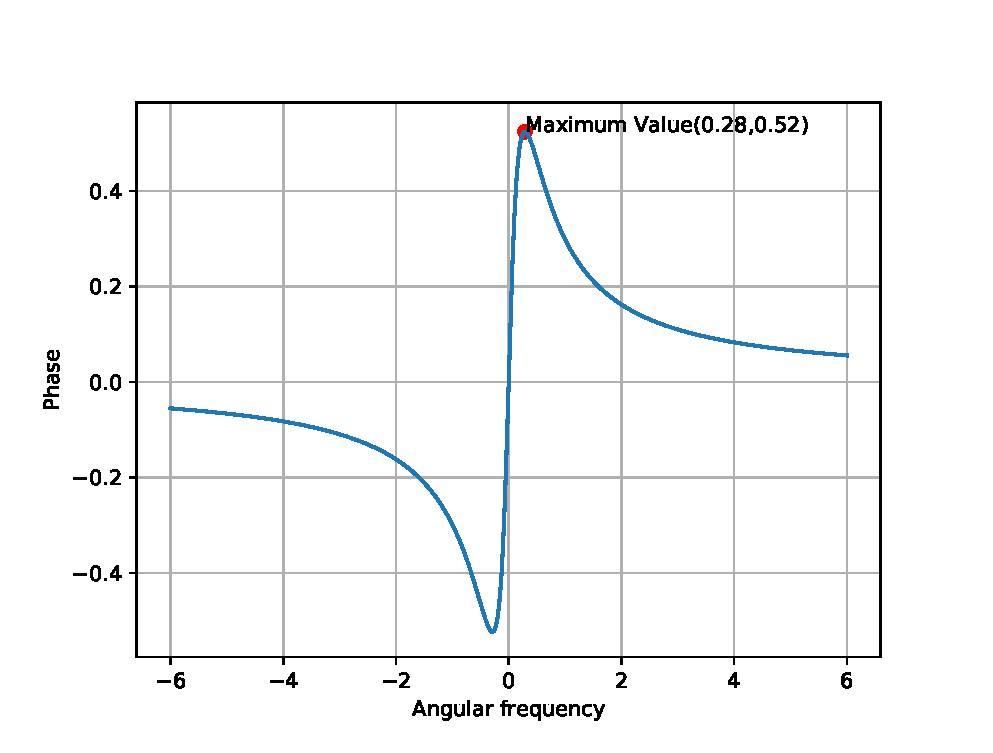
\includegraphics[width=\columnwidth]{./figs/ee18btech11010.eps}
	\caption{}
	\label{fig:ee18btech11010}
\end{figure}
 
\textbf{Applications:}\\ \\
\begin{enumerate}
  \item Phase lead Compensators can be used as High pass filters,Differentiators.
  \item They are used to reduce steady state errors. 
  \item Increases Phase Margin , relative stability.
\end{enumerate}
\item What is purpose of of a Phase Lead Compensator?
\item Through an example, show how the compensator in Problem \ref{prob:ee18btech11010_comp} can be used in a control system.



\end{enumerate}


